%%%%%%%%%%%%%%%%%%%%%%%%%%%%%section Boundary Conditions%%%%%%%%%%%%%%%%%%%%%%%%%%%%%%%%%%%%%%%%%%%%%%%%%%%%%%%%%%%%
%%%%%%%%%%%%%%%%%%%%%%%%%%%%%%%%%%%%%%%%%%%%%%%%%%%%%%%%%%%%%%%%%%%%%%%%%%%%%%%%%%%%%%%%%%%%%%%%%%%%%%%%%%%%%%%%%%
\section{Boundary Conditions}\label{sec:BC}
%%%%%%%%%%%%%%%%%%%%%%%%%%%%%%%%%%%% subsection General introduction to boundary conditions %%%%%%%%%%%%%%%%%%%%%%%%%%%%%%%%%%%%%%%%%%%%%%%%%%%%%%%%%%%%%%%%%%%%%
    \subsection{General introduction to boundary conditions}\label{subsec:General introduction to BC}
    \subsubsection{Equations of boundary conditions}\label{subsubsec:Equations of BC}
	  Boundary conditions (BC) are necessary for solving the  Maxwell's equations by FDTD. They can limit the computation in a finite space but attaining the same solution just as in a infinite one.  \\
	  The following equations are the general boundary conditions at an arbitrary interface of two medium. And there can be  charges (denoted as charge density $\rho_s$) or  currents (denoted as surface electric current density $\vec{\mathbf{J}}_s$ and  surface magnetic current density $\vec{\mathbf{M}}_s$) at the interface:
	  %%%%% BC EQ
	      \begin{eqnarray}
		  \hat{n}\cdot(\vec{\mathbf{D}}_2-\vec{\mathbf{D}}_1) &=&\rho_s  \\
		  \hat{n}\cdot(\vec{\mathbf{B}}_2-\vec{\mathbf{B}}_1) &=&0  \\
		  \hat{n}\times(\vec{\mathbf{E}}_2-\vec{\mathbf{E}}_1) &=&-\vec{\mathbf{M}}_s \\
		  \hat{n}\times(\vec{\mathbf{H}}_2-\vec{\mathbf{H}}_1) &=&\vec{\mathbf{J}}_s
		  \label{eq:General boundary conditions}
	      \end{eqnarray}
      %     %%%%% BC Diagrams
      %     Figure  \ref{fig:General BC diagrams} shows the above relations.
      %     \begin{figure}[ht]
      %       \centering
      % 	  %\subfloat[CAPTION]{BILDERCODE}\qquad
      % 	  \subfloat[$\vec{\mathbf{D}}$]{\includegraphics[width=0.4\textwidth]{svg/BC_general_Dn.eps}}\qquad
      % 	  \subfloat[$\vec{\mathbf{B}}$]{\includegraphics[width=0.4\textwidth]{svg/BC_general_Bn.eps}}\qquad 
      % 	  \subfloat[$\vec{\mathbf{E}}$]{\includegraphics[width=0.4\textwidth]{svg/BC_general_Et.eps}}\qquad
      % 	  \subfloat[$\vec{\mathbf{H}}$]{\includegraphics[width=0.4\textwidth]{svg/BC_general_Ht.eps}}\qquad 
      % 	    \caption[General BC diagrams]{General boundary condition on an interface between 2 media for $\vec{\mathbf{D}}$, $\vec{\mathbf{B}}$, $\vec{\mathbf{E}}$ and $\vec{\mathbf{H}}$. n denotes normal components. t denotes tangential components. s denotes surface.}
      % 	    \label{fig:General BC diagrams}
      %     \end{figure}
    \subsubsection{Four particularly useful types of boundary conditions in OpenEMS}\label{subsubsec:Four particularly usefull BC}
	Under some special given conditions or assumptions, the boundary conditions(\ref{eq:General boundary conditions}) have  respective forms and they are convenient for the most simulations. These BC are called as perfect electric conductor (\textbf{PEC}), perfect magnetic conductor (\textbf{PMC}), \textbf{MUR} absorbing boundary condition and perfectly matched layer (\textbf{PML}) absorbing boundary condition. More details of these four types of BC are  given in the following subsections (\ref{subsec:PEC}, \ref{subsec:PMC}, \ref{subsec:MUR} and  \ref{subsec:PML}). And the types of these BC are represented as a field of the structure  \hyperref[para:FDTD]{\texttt{FDTD}} in MATLAB. And it's named as \texttt{BoundaryCond}. \phantomsection \label{para:BoundaryCond}
    \subsubsection{Setting boundary conditions in OpenEMS with function SetBoundaryCond}\label{subsubsec:Setting boundary conditions in OpenEMS with function SetBoundaryCond}
	\textcolor{blue}{\begin{large}\textbf{SetBoundaryCond}	\end{large}}\\
	  Setting boundary conditions for simulation. Assigning the field \hyperref[para:BoundaryCond]{\texttt{BoundaryCond}} of structure \hyperref[para:FDTD]{\texttt{FDTD}}  in MATLAB.

        \textcolor{blue}{\begin{large}Syntax:\end{large}}
 \begin{lstlisting}
FDTD = SetBoundaryCond(FDTD, BC)
%or with advanced arguments
FDTD = SetBoundaryCond(FDTD, BC, varargin)
 \end{lstlisting}

	\textcolor{blue}{\begin{large}Description:\end{large}}\\
	\hyperref[para:FDTD]{\texttt{FDTD}}
  \begin{myindentpar}\hyperref[para:FDTD]{\texttt{FDTD}}  is a structure in Matlab. It contains 3 fields:
       \begin{myindentpar}\texttt{ATTRIBUTE} \\
	      \texttt{Excitation} \\
	      \texttt{BoundaryCond}
      \end{myindentpar}
  \end{myindentpar}
%%%%%%%%%%%%%%%%%%%%%%%%%%%% BC
	\texttt{BC}  
\begin{myindentpar}\texttt{BC} provides the types of the boundary conditions to the 6 boundaries of the 3D simulating space.  
          \texttt{BC} is defined either as a \textbf{vector} or as a \textbf{cell} with 6  elements. \vspace{2mm}\\
          If  T\_xmin,T\_xmax,T\_ymin,T\_ymax,T\_zmin and T\_zmax are  arguments which denote for the types of the conditions at the respective boundaries, then \texttt{BC} can be defined as a vector or a cell as following.\vspace{2mm}\\
       %%%%%%%%%%%% vector BC
          \texttt{BC} is defined as a \textbf{vector}
	\begin{myindentpar}
% 	  \lstset{caption={\texttt{BC} in the form of a vector},label=BCinvector}
	  \begin{lstlisting}[caption={\texttt{BC} in the form of a vector},label=BCinvector]
 BC=[T_xmin T_xmax T_ymin T_ymax T_zmin T_zmax]; 
	  \end{lstlisting}
          And   each  element(T\_?min or T\_?max)  must be set as one of the following numbers 
	    \begin{myindentpar}
	      \textcolor{green}{\texttt{0}}   \qquad  (represents for PEC)\\
	      \textcolor{green}{\texttt{1}}   \qquad  (represents for PMC)\\
	      \textcolor{green}{\texttt{2}}   \qquad  (represents for MUR)\\
	      \textcolor{green}{\texttt{3}}   \qquad  (represents for PML with 8 layers).
	    \end{myindentpar}	
      \end{myindentpar}  
          %%%%%%%%%%%% Cell BC      		                                                                     
          Or \texttt{BC} is defined as a \textbf{cell} 
	  \begin{myindentpar}
% 	   \lstset{caption={\texttt{BC} in the form of a cell},label=BCincell}
	  \begin{lstlisting}[caption={\texttt{BC} in the form of a cell},label=BCincell]
 BC={T_xmin T_xmax T_ymin T_ymax T_zmin T_zmax};
	  \end{lstlisting}
	  of which   each  element(T\_?min or T\_?max)  must be set as one of the following strings 
	  \begin{myindentpar}
	     \textcolor{green}{\texttt{'PEC'}} \qquad   (represents for PEC)\\
	     \textcolor{green}{\texttt{'PMC'}} \qquad   (represents for PMC)\\
	     \textcolor{green}{\texttt{'MUR'}}  \qquad  (represents for MUR)\\
	     \textcolor{green}{\texttt{'PML\_x'}} \qquad   (represents for PML. \texttt{x} is  the PML size. It should be replaced with an integer in an interval from 4 to 50).
	  \end{myindentpar}	
	\end{myindentpar}	
	  So the element \texttt{BC}($i$) or \texttt{BC}\{$i$\} represents for the type of the  condition at the respective boundary as showed in the following table
	  \begin{table}[htb]\centering
	  \begin{tabular}{l|l}
	  \texttt{BC($i$)} or \texttt{BC\{$i$\}} & Respective position of the boundary\\ \hline
		 \texttt{BC(1)} or  \texttt{BC\{1\}} & where x or $\rho$ is minimum\\
		 \texttt{BC(2)} or  \texttt{BC\{2\}}& where x or $\rho$ is maximum\\
		 \texttt{BC(3)} or  \texttt{BC\{3\}}& where y or $\varphi$ is minimum\\
		 \texttt{BC(4)} or  \texttt{BC\{4\}}& where y or $\varphi$is maximum\\
		 \texttt{BC(5)} or  \texttt{BC\{5\}}& where z is minimum\\
		 \texttt{BC(6)} or  \texttt{BC\{6\}}& where z is maximum
	  \end{tabular}\caption{The elements represent for the types of conditions at the boundaries.}
	  \end{table}
	  \label{Elements of BC and the rescpective boundaries}.
         \end{myindentpar}
            %%%%%%%%%%%%%%%% Info 
	\info{In a cylindrical system,  the elements of \texttt{BC} represent for the types of boundaries conditions respective at $\rho$, $\varphi$, z instead of x, y, z(see listing \ref{ListingCylinBC}). If there are no  BC at $\rho\_min=0$ or at $\varphi$,  then the elements of  \texttt{BC} for respective boundaries conditions   can be set as \texttt{0} or \texttt{'PEC'} just in a virtual form for computation(see listing \ref{listing:SettingofBC in a cylin.}). For these cases, the respective elements have nothing to do with the boundaries conditions indeed. } \\
% 	  \lstset{caption={\texttt{BC} in a cylindrical coordinate},label={ListingCylinBC}}
         \begin{lstlisting}[caption={\texttt{BC} in a cylindrical coordinate},label={ListingCylinBC}]
% as a vector
  BC=[T_rhomin T_rhomax T_phimin T_phimax T_zmin T_zmax];
% as a cell
  BC={T_rhomin T_rhomax T_phimin T_phimax T_zmin T_zmax}
	  \end{lstlisting}%%question: phi_min and phi_max don't form a closed circle,then???
%%%%%%%%%%%%%%%%%%%%%% varargin
	      Advanced arguments \texttt{Varargin}:
      \begin{myindentpar} \texttt{Varargin}  are  arguments of advanced settings. They can be either neglected or replaced with the following alternative arguments  
		\begin{myindentpar}
		  \textcolor{green}{\texttt{'MUR\_PhaseVelocity'}}\\
		  \textcolor{green}{\texttt{'PML\_Grading'}}\\
		  \textcolor{green}{\texttt{'gradFunction'}}.
		\end{myindentpar}
      and respective values following them.\vspace{2mm}\\
			%%%%%%%%%%%%%% MUR
		\texttt{'MUR\_PhaseVelocity'} 
		  \begin{myindentpar}
		      It defines a phase-velocity to be used by the MUR-abc
		      useful e.g. for dispersive waveguides
		  \end{myindentpar}
	    \vspace{2mm} 
			%%%%%%%%%%%%%%% PML
	      \texttt{'PML\_Grading'} or \texttt{'gradFunction'} 
		\begin{myindentpar}
		They define the PML grading function.\vspace{2mm}
			    Predefined variables in this grading function are:
			      \begin{myindentpar}
				D  = depth in the pml in meter\\
				dl = mesh delta inside the pml in meter\\
				W  = width (length) of the pml in meter\\
				N  = number of cells for the pml\\
				Z  = wave impedance at the current depth and position
			    \end{myindentpar}
		\end{myindentpar}
      \end{myindentpar}

%%%%%%%%%%%%%%%%%%%%% Examples.	  
	\textcolor{blue}{\begin{large}Examples:\end{large}}\\
\begin{itemize}
%%%%%%%1st step
 \item    Setting boundaries conditions in a Cartesian coordinate system.\\
       1st step: \texttt{BC} assignment
    \begin{myindentpar}
	  \begin{lstlisting}[caption={BC assignment as fig \ref{fig:Ex. 1st of SetBoundaryCond} },label={listing:1st SettingofBC}]
	  %using numbers 
	  BC=[ 1     1     0     0     2     3     ] 
	  %or using equivalent strings
	  BC={'PMC' 'PMC' 'PEC' 'PEC' 'MUR' 'PML_8'} 
		      \end{lstlisting}
	  Both above vector and cell set  the x-boundaries(perpendicular to x axis) as PMC, and the y-boundaries(perpendicular to y axis) as PEC, the zmin-boundary(perpendicular to z axis and z is minimum) as MUR but the zmax-boundary(perpendicular to z axis and z is maximum) as PML with 8 layers. These boundary condition are showed in fig \ref{fig:Ex. 1st of SetBoundaryCond}.
	      \begin{figure}[ht]
		      \centering
		    \subfloat[BC at x and y]{\includegraphics[width=0.4\textwidth]{svg/BCXY1.eps}}\qquad
		    \subfloat[BC at x and z]{\includegraphics[width=0.4\textwidth]{svg/BCXZ1.eps}}\qquad 
%\includegraphics[width=0.9\textwidth]{svg/BCXY.eps}
		      \caption[1st example for the setting of boundaries conditions]{\texttt{BC=[1 1  0 0  2 3]} ,see listing \ref{listing:1st SettingofBC}}
		      \label{fig:Ex. 1st of SetBoundaryCond}
		\end{figure}
    \end{myindentpar}
%%%%%%%2nd step
      2nd step: Updating the \hyperref[para:FDTD]{\texttt{FDTD}} structure with BC or other andvanced arguments.
      \begin{myindentpar}	    
		    \begin{lstlisting}
  % without advanced arguments
  FDTD=SetBoundaryCond(FDTD,BC); 
		    \end{lstlisting}
		      or
		    \begin{lstlisting}
  % with advanced argument for MUR
  FDTD=SetBoundaryCond(FDTD,BC,...
       'MUR_PhaseVelocity',300000000);
			\end{lstlisting}
		    \begin{lstlisting}
  % with advanced argument for PML
  FDTD=SetBoundaryCond(FDTD,BC,...
       'PML_Grading','-log(1e-6)*log(2.5)/...
       (2*dl*pow(2.5,W/dl)-1)*pow(2.5, D/dl)/Z');
		    \end{lstlisting}	 
    \end{myindentpar}	
%%%%%%%%%% cylindrical sys
 \item Setting boundaries conditions in a cylindrical coordinate system.\\
If there are no boundaries at  $\rho_{min}=0$ and at any $\varphi$, then please set the elements as \texttt{0} or \texttt{'PEC'} as the following example.
    \begin{lstlisting}[caption={BC assignment in a cylindrical coordinate system as fig \ref{fig:Ex. SetBoundaryCond in cylin.}},label={listing:SettingofBC in a cylin.}]
	% no boundaries at rhomin=0 , phi_min and phi_max
	BC=[0 1 0 0 3 3];
	%or using equivalent strings
	%BC={'PEC' 'PMC' 'PEC' 'PEC' 'PML_8' 'PML_8'} 
	FDTD=SetBoundaryCond(FDTD,BC); 
			\end{lstlisting} 
    \begin{figure}[ht]
			  \centering
			\includegraphics[width=0.6\textwidth]{svg/CylinBCXY.eps}\qquad
			  \caption[ Setting virtual boundaries conditions in a cylindrical coordinate system]{Virtual boundaries conditions in a cylindrical coordinate system. See listing \ref{listing:SettingofBC in a cylin.}}
			  \label{fig:Ex. SetBoundaryCond in cylin.}
		    \end{figure}
%%%%%%%%%%%%% half cylindrical
If there are boundaries at $\rho_{min}\neq0$ and $\varphi$, then please set the elements as respective number or string.
\begin{lstlisting}[caption={BC assignment in a cylindrical coordinate system as fig \ref{fig:Ex. SetBoundaryCond in cylin. Half}},label={listing:SettingofBC in a cylin. Half}]
	% no boundaries at rhomin=0 , phi_min and phi_max
	BC=[0 1 0 1 0 3];
	%or using equivalent strings
	%BC={'PEC' 'PMC' 'PEC' 'PMC' 'PEC' 'PML_8'} 
	FDTD=SetBoundaryCond(FDTD,BC); 
			\end{lstlisting} 
    \begin{figure}[H]
			  \centering
 \subfloat[Boundaries conditions at $z$  ]{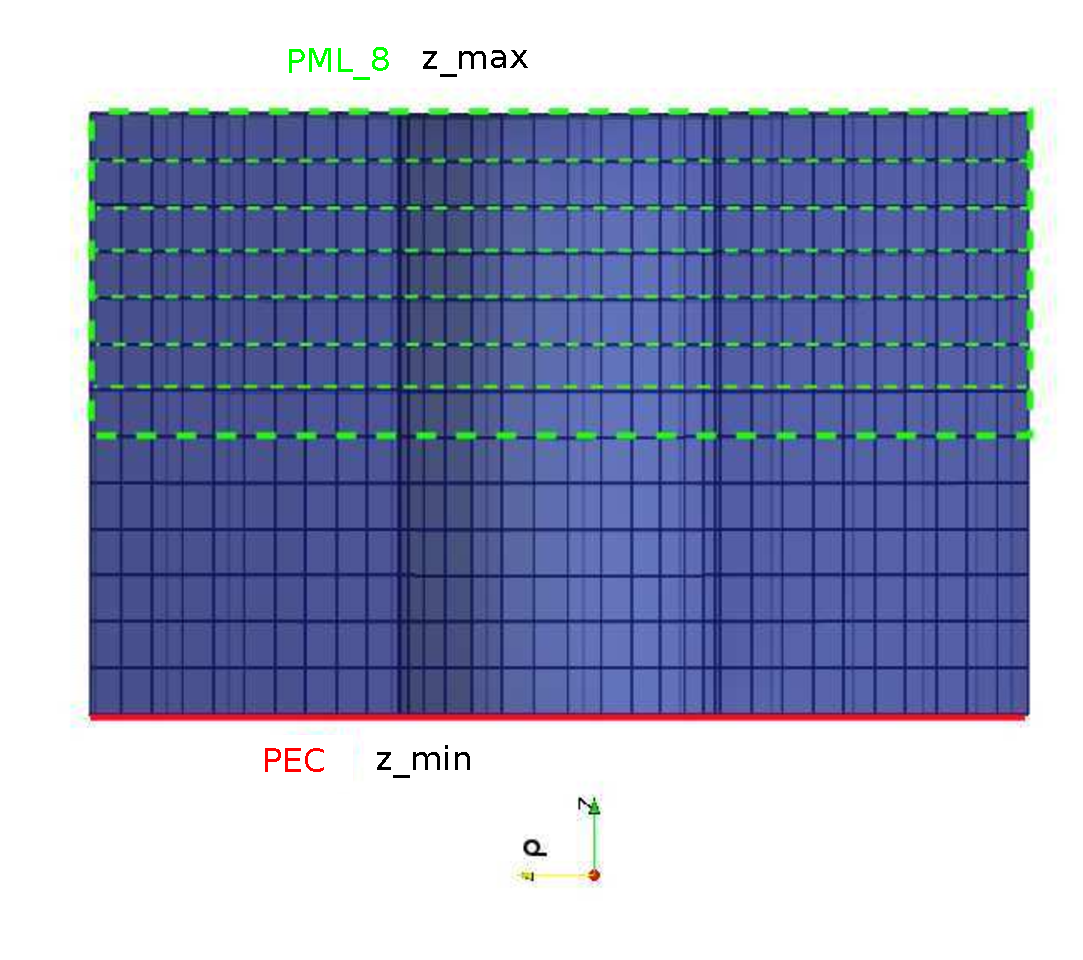
\includegraphics[width=0.6\textwidth]{svg/CylinBCXZ2.eps}}\qquad
 \subfloat[ Boundaries conditions at $\rho$ and $\varphi$ ]{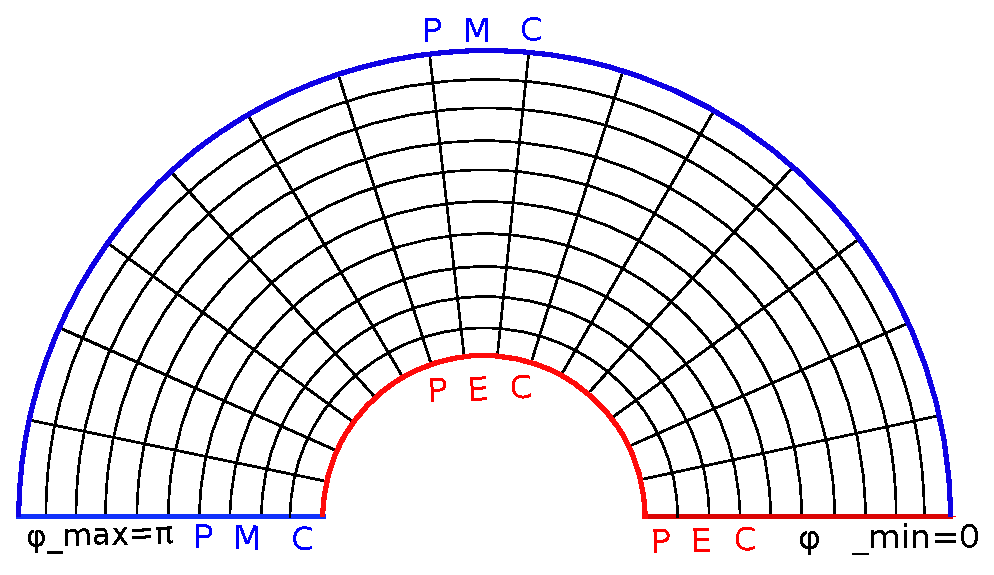
\includegraphics[width=0.55\textwidth]{svg/CylinBCXY2.eps}}\qquad 
			  \caption[ Setting  boundaries conditions in a cylindrical coordinate system]{An example of boundaries conditions in a cylindrical coordinate system. See listing \ref{listing:SettingofBC in a cylin. Half}}
			  \label{fig:Ex. SetBoundaryCond in cylin. Half}
		    \end{figure}
\end{itemize}
%%%%%%%%%%%%%%%%%%%%%%%%%%%%%%%%%%%% subsection Perfect electric conductor (PEC) %%%%%%%%%%%%%%%%%%%%%%%%%%%%%%%%%%%%%%%%%%%%%%%%%%%%%%%%%%%%%%%%%%%%%
    \subsection{Perfect electric conductor (PEC)}\label{subsec:PEC}
    \subsubsection{Definition of PEC}
    If one media beside the boundary is theoretically lossless(conductivity $\sigma\rightarrow\infty$, or so called \textbf{perfect conductor}), then the BC can be expressed as
	%%%%% PEC BC EQ
	    \begin{eqnarray}
		\hat{n}\cdot\vec{\mathbf{D}}_1 &=&-\rho_s  \\
		\hat{n}\cdot\vec{\mathbf{B}}_1 &=&0  \\
		\hat{n}\times\vec{\mathbf{E}}_1 &=&0\\
		\hat{n}\times\vec{\mathbf{H}}_1 &=&-\vec{\mathbf{J}}_s .
		\label{eq:PEC boundary conditions}
	    \end{eqnarray}
    \subsubsection{The condition for application of PEC}
    In practice, this BC can be applied where the media  is \textbf{good conductor(e.g., metal)}, because the good conductor can often be seen as nearly lossless(perfect). So condition for using PEC can be summarized as either
    \begin{itemize}
    \item one media is good conductor(e.g., metal) \\
    or
    \item $\sigma\rightarrow\infty$.
    \end{itemize}
    \subsubsection{The Setting of PEC in OpenEMS}

    %     %%%%% PEC BC Diagrams
    %     Figure  \ref{fig:PEC BC diagrams} shows the above relations.
    %     \begin{figure}[ht]
    %             \centering
    % 	    \includegraphics[width=0.4\textwidth]{svg/PEC_BC_general_Dn.eps}
    % 	    \caption[PEC BC diagrams]{PEC boundary condition  for $\vec{\mathbf{D}}$, $\vec{\mathbf{B}}$, $\vec{\mathbf{E}}$ and $\vec{\mathbf{H}}$. n denotes normal components. t denotes tangential components. s denotes surface.}
    % 	    \label{fig:PEC BC diagrams}
    %     \end{figure}
\warning{The first or last layer of nodes of E field in the boundary can not be updated, because there are no enough nodes of H field around them for calculation. So the field there should be neglected.}

%%%%%%%%%%%%%%%%%%%%%%%%%%%%%%%%%%%%%%%%%%%%%%%%% subsection Perfect magnetic conductor (PMC) %%%%%%%%%%%%%%%%%%%%%%%%%%%%%
\subsection{Perfect magnetic conductor (PMC)}\label{subsec:PMC}
H perpendicular to BC

%%%%%%%%%%%%%%%%%%%%%%%%%%%%%%%%%%%%%%%%%%%%%%%%% subsection MUR absorbing boundary condition %%%%%%%%%%%%%%%%%%%%%%%%%%%%%
\subsection{MUR absorbing boundary condition}\label{subsec:MUR}

%%%%%%%%%%%%%%%%%%%%%%%%%%%%%%%%%%%%%%%%%%%%%%%%% subsection Perfectly matched layer (PML) absorbing boundary condition %%%%%%%%%%%%%%%%%%%%
\subsection{Perfectly matched layer (PML) absorbing boundary condition}\label{subsec:PML}
matched--impedance ,no reflection , for infinite  material, an virtual BC for computation
\warning{Since the field is absorbed in the boundary artificially, please pay attention to any setting in these region. For example, don't place any excitation in it. And please set enough layers of meshes, such that the boundary works correctly.}

